\documentclass[tikz,border=2mm]{standalone}
\usetikzlibrary{trees,positioning}

\begin{document}

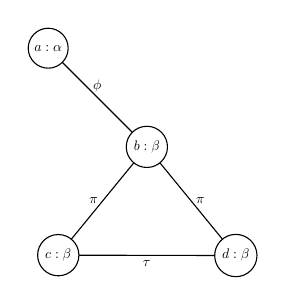
\begin{tikzpicture}[scale=0.5,
	vertex/.style={circle, draw, minimum size=1cm},
	every edge/.style={draw},
	transform shape
]

	% Vertices
	\node[vertex] (a) {$a:\alpha$};
	\node[vertex, below right=2.5cm of a] (b) {$b:\beta$};
	\node[vertex, below left=2cm and 1.5cm of b] (c) {$c:\beta$};
	\node[vertex, below right=2cm and 1.5cm of b] (d) {$d:\beta$};

	% Edges with labels
	\draw (a) -- node[above] {$\phi$} (b);
	\draw (b) -- node[left] {$\pi$} (c);
	\draw (b) -- node[right] {$\pi$} (d);
	\draw (c) -- node[below] {$\tau$} (d);

\end{tikzpicture}

\end{document}
